%!TEX root = bioPrediction_main.tex
\section{Field Study}
We conducted an eight-week field study with 14 participants using experience sampling and biometric sensors to investigate how knowledge workers experience stress \rev{and awakeness} over time and the feasibility of predicting stress, focus, and awakeness \rev{using} biometric signals. 


\subsection{Participants}
We recruited a group of 14 professionals via personal contacts from a large power and automation company. The group is diverse in terms of age, work experience, gender, and work responsibilities. All participants work primarily in an office environment, though half of the participants spend at least 10\% (and up to 50\%) of their time in a laboratory environment. Office workers are a population that generalizes to a variety of contexts, including part-time laboratory workers, and guarantees that our participants have varying work patterns that include different levels of computer usage, as well as different levels of activity in both individual and collaborative tasks.

From the 14 participants, 11 are male and 3 are female. The average participant age is ~40, with 5 in the age range 25-34, 7 in the age range 35-44, and 2 in the age range 55+. The average number of years of professional experience of the participants is 12, with 2 having less than 5 years, 10 having 5-15 years, and 2 having more than 25 years. All participants work for a research organization within the company, but their job functions span line management, laboratory science, scientific research, technology evaluation, and software development.


\subsection{Procedure}
We performed a study over the course of eight weeks. This study includes the collection of the participant's \rev{biometric data and self-reporting surveys during their work hours}. \rev{We also collected computer interaction data, but given privacy concerns of some participants chose not to use this data (see Section~\ref{sec:computer_interaction_data})}. We informed participants about the study purpose and procedure, handed out biometric sensors, introduced and explained the self-reporting to the participants, \rev{handed out consent forms and ensured informed consent from each participant for the study.}


After the initial setup, participants were asked to fill out three surveys each day for the following eight weeks (see Section~\ref{sec:Surveys}) \rev{and wear the biometric sensor during their work hours}. At the end of the eight weeks, we collected the biometric sensors and performed a short follow-up interview on the study and the participants' experiences.

Keeping participants engaged in an eight-week study can be
difficult. In the second month of the study, largely to incent participants to
continue, we offered participants two one-hour Tai Chi classes per
week (each in the middle of the day) and asked them to attend one
class a week. The choice of Tai Chi provided a link to mindfulness,
a topic of growing interest in communities. Consultations we held
with researchers in psychiatry and psychology suggested Tai Chi as
a good link to mindfulness and an intervention that might alleviate
stress. By recording attendance of participants at the Tai Chi
sessions, we are able to analyze the impact of the sessions
on the results. As a brief summary, the impact of the
sessions was minimal; we present an analysis
of the effects in Section~\ref{sec:Discussion}.

%\tfC{What's missing is when we asked participant to wear it. Chris: do you know what the usual time window of the Everion data was? we could state that here or in section 2.3. this would mitigate the question on shower usage since I think we only asked them to wear it during working hours, but I'm not sure anymore :(.}

\begin{comment}
%\subsection{Procedure}
%\todo{This section does not work here. It is not really the study procedure, but rather the project procedure. Perhaps it can form the basis of an overview section after Field Study but before Analysis and Results.}

%\begin{figure}
%  \centering
%      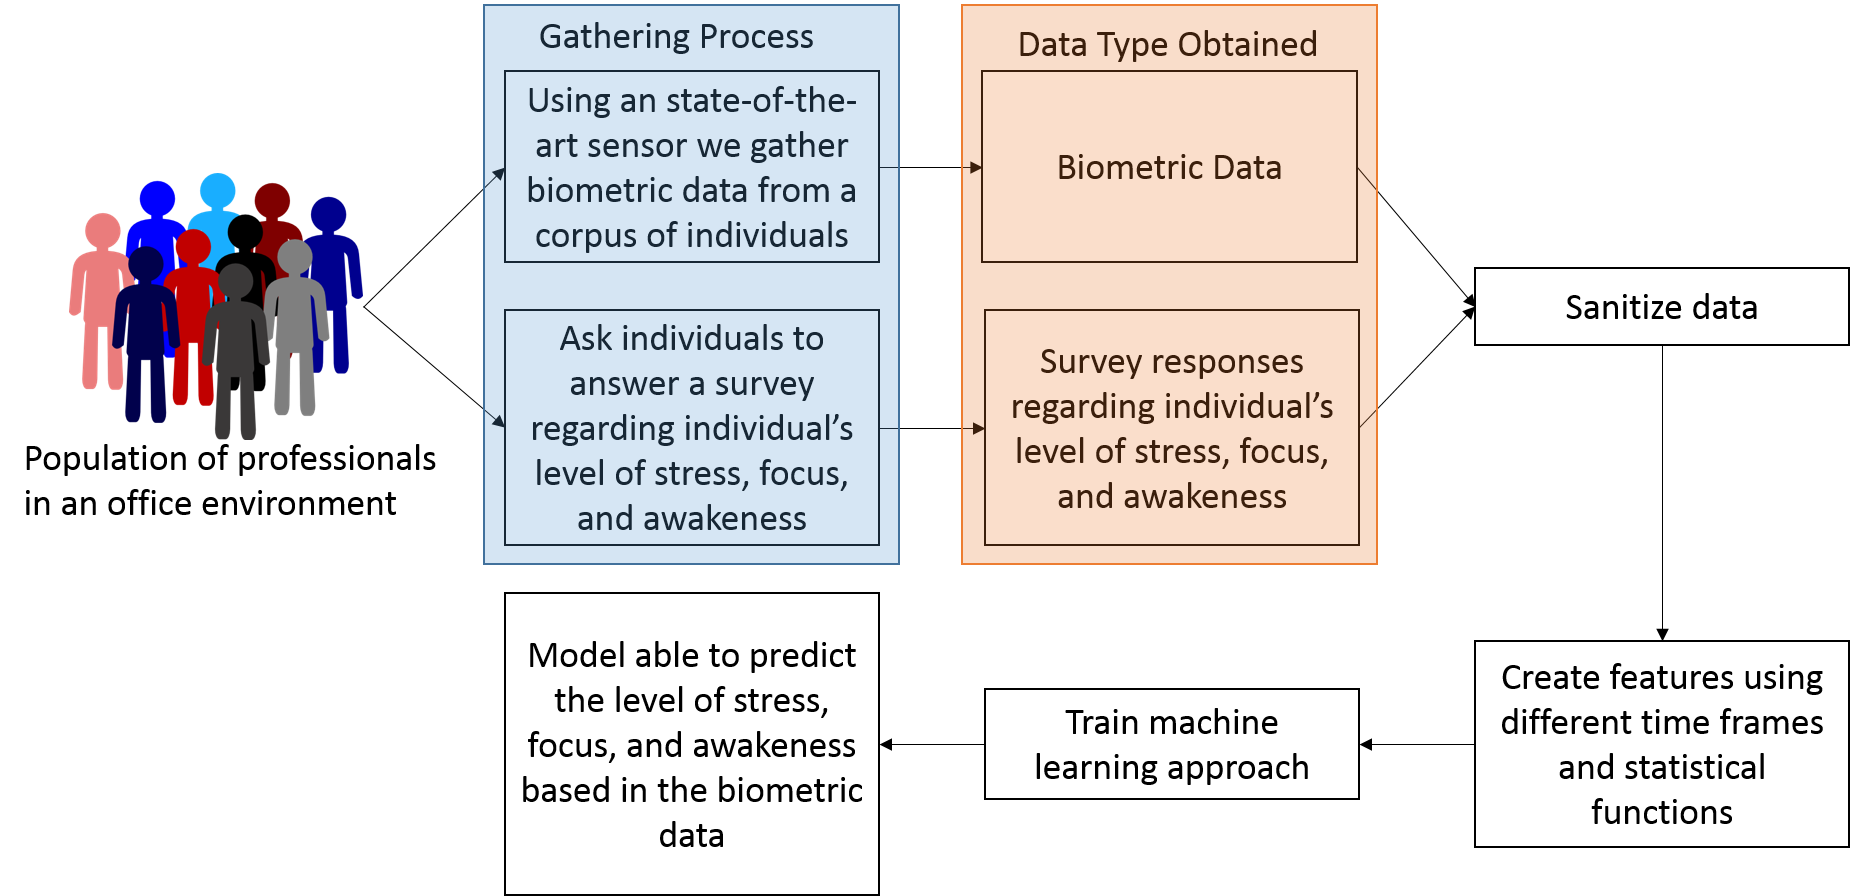
\includegraphics[width=0.5\textwidth]{Figure1.png}
%  \caption{Process used to gather data and create the machine learning model able to predict the level of stress, focus, and awakeness} 
%  \label{process}
%\end{figure}
%\todo{The figure or text in the boxes could be shortened a lot, maybe even just replaced with pictures of sensor and survey like question with 5point scale. At this point, i'm not sure the figure adds a lot.}

%Figure \ref{process} shows the overall process performed in this study. We started by selecting a population
%of professionals in an office environment.

%We use state-of-the-art sensors to capture a stream of biometric data from each individual and a computer interaction tracker to collect computer interaction information during the time
%of the study. 

%The participants were asked to fill a survey 3 times a day: two during the working day, and
%one at the end of the day, where they rated their level of stress, focus, and awakeness during
%the day; and their level of stress, awakeness, productiveness, and overall feeling at the end of the day.
%This was conducted over an eight week period, which is
%400\% longer than previous studies~\cite{zuger18,Muller16}.

%We then pick a set of time windows (10sec, 20sec, 30sec, 45sec, 1min, 2min, 3min, 5min, 7.5min, 10min, 20min, 30min, 45min, 1hour, 2hour, 3hour) to analyze. We applied different statistical measurements (mean, standard deviation, variance, median, percentile25, percentile75, interquartile range, maximum, minimum, range) to each of the collected biometric signals and the computer interaction data within the time windows selected. We then 
%compared the performance of four different machine learning 
%algorithms to be able to predict the survey responses based in the biometric and 
%computer interaction data.

%Based in the initial corpus of training data, we create a machine learning model that is able to accurately predict the responses for stress, focus, and awakeness for each of the individuals wearing the sensors.
%We are therefore able to infer the answer within the spectrum to each of these indicators without the need to ask the participants to provide an answer.
\end{comment}

\subsection{Data Collection}
\label{sec:DataCol}
We collected two datasets  from each study participant.

\subsubsection{Biometric Sensors}
Figure~\ref{everion} illustrates Biovotion's Everion, which we used to track the biometric signals of the study participants. The Everion is worn on the upper arm and provides continuous monitoring of certain biometric measurements.\footnote{https://biovotion.zendesk.com/hc/en-us/articles/213613165} Previous studies~\cite{zuger18,sano2013stress,healey2005detecting,wijsman2011towards,zuger2015interruptibility,goyal2017intelligent} have used similar devices~\cite{Okada11,polar,fitbitCharge} to capture psycho-physiological and biometric measurements for shorter periods of time or capturing a smaller number of measurements.
\rev{A comparative study has  shown that the Everion can be used as a valid proxy for HRV metrics for knowledge workers~\cite{barrios2019a}.} 

\begin{figure}
  \centering
      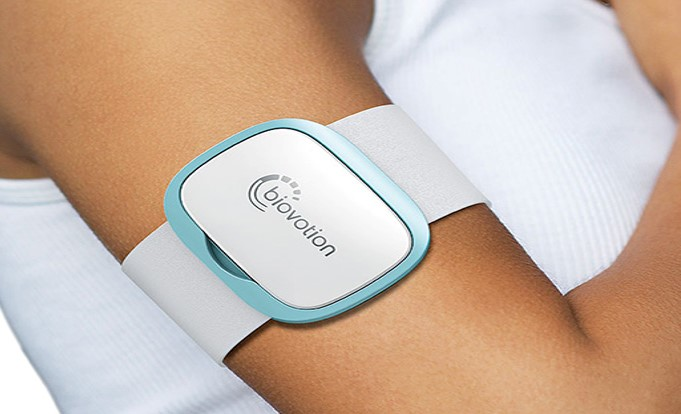
\includegraphics[width=0.5\textwidth]{Everion.jpg}
  \caption{We used Biovotion's Everion to collect biometric measurements from the participants}
   \label{everion}
\end{figure}

Table~\ref{signals} lists the biometrics measurements that we collected using the Everion. Each measurement is collected once per second, and each recorded observation has an associated timestamp and quality rating. Data collected by the Everion are uploaded to a server, from which we downloaded the data for use in our study. \rev{We chose these biometric measurements based on previous research that has indicated their potential (see references in Table~\ref{signals}) and the availability and feasibility of collecting these measurements with low invasiveness over a long duration.} 



\begin{table}[h!]
\begin{center}
\small\addtolength{\tabcolsep}{10pt}%-1pt}
\begin{tabular}{l l}
\hline
Biometric Measurement & Units of Measure \\ 
\hline
\textbf{Physical Activity} & \cite{fox1999,aldana1996}\\
\hspace{3mm}Intensity of motion & (No unit)  \\
\hspace{3mm}Energy Expenditure & Calories per second (cal/s)  \\
\hspace{3mm}Step counter & Steps  \\
\hline
\textbf{Heart} & \cite{haapalainen2010psycho,healey2005detecting,mulder1992measurement,haag2004emotion} \\
\hspace{3mm}Heart rate & Beats per Minute (bpm) \\
\hspace{3mm}Blood pulse wave & (No Unit)  \\
\hspace{3mm}Heart rate variability: RMSSD  & Milliseconds (ms) \\
%\multicolumn{2}{l}{\hspace{4mm}\textit{(RMSSD: root mean square of successive heartbeat interval differences)}} \\
\hspace{3mm}Blood oxygenation  & Percent (\%)  \\
\hspace{3mm}Blood perfusion & (No unit)  \\
\hline
\textbf{Skin} & \cite{healey2005detecting,haag2004emotion} \\
\hspace{3mm}Galvanic skin response &  kOhm  \\
\hspace{3mm}Skin temperature &  Degrees Celsius ($^{\circ}$C)  \\
\hline
\textbf{Respiration} & \cite{mulder1992measurement,healey2005detecting,haag2004emotion,masaoka1997}\\
\hspace{3mm}Respiratory rate & Breaths per Minute (bpm)  \\
\hline
%\textbf{Environmental}\\
%\hspace{3mm}Barometric pressure & Milibar (mbar)  \\
%\hline
\end{tabular}
\caption{Biometric measurements captured by the Everion, organized by category and with references to previous works using similar data. \rev{\textit{(RMSSD denotes the root mean square of successive heartbeat interval differences)}}}
\label{signals}
\end{center}
%\vspace*{-4mm}
\end{table}

\subsubsection{Computer Interaction Data}\label{sec:computer_interaction_data}
To gain a better understanding of our participants day-to-day work activities, we \rev{asked participants to install} an open source computer interaction monitor~\cite{Meyer17}. The monitor ran in the background on participants' computers and tracked the active windows, as well as the keyboard and mouse activity. Four of our participants opted out of this part of the study for privacy reasons (S6, S10, S12, and S13).
% Gail: I commented out Thomas' comment as I don't think we need to address it
%\tfC{Probably needs to state something about how it also captured non-work related browsing (see section 3.4)}
%Therefore, we only included the computer interaction data in our analysis for our more coarse-grained explanatory model but not in our analysis on the predictive model for stress in the moment. 

\subsubsection{Surveys}
\label{sec:Surveys}
Following guidelines from previous studies~\cite{Lalle16,Panwar18,Luo18} and 
following the preferences of extensive user piloting, we sent via 
text message a survey request to each participant two times per 
work day. Pilot participants preferred the usage of text message, in part, due 
to them being accessible and noticeable anywhere in the office. 

We sent the 
first request at a random time between 9am and 11am 
and sent the second request at a random time between 1pm and 3pm. We 
randomized the request times to avoid either establishing or observing a 
standard behavioral pattern. That is, we did not want the participants to 
plan for the arrival of the survey request at a set time, and we did not 
want the survey request to overlap with a set daily behavior (e.g., coffee 
break every day at 2:30pm). Similarly, we avoided using tools which allow 
for too much freedom in response time~\cite{Adams18} since this would 
discourage participation in stressed time frames and would bias the 
corpus. 
%This sentence was added in response to Reviewer 1 comment:
%There is already a lot of work on designing a new self-log, a self-report 
%tool which can blend into the workstation [1] or offers users more freedom 
%in time to self-report [2], or facilitate the self-log by using wearables.
The same survey was sent each time:
\begin{enumerate}
\item How awake are you right now?
\item How stressed do you feel right now?
\item How focused on work are you right now? 
\end{enumerate}
We used the phrase ``right now'' to capture each aspect in the moment (so as to permit later prediction of each aspect based on biometric data). The wordings of the questions are based on a previous survey of individuals in an organizational context~\cite{Gloor_etal:2010}. The use of awakeness (rather than sleepiness) in Question 1 is inspired by previous work~\cite{Wilhelm_Schoebi:2007} and to some extent also captures the ``arousal'' aspect of the affective space~\cite{Russell:1980}.


%\todo{we are not using the last survey for anything in this paper, so I'd leave it out}
One last survey was sent at the end of the day, at 4:25pm which asked the 
four different questions
detailed below:
\begin{enumerate}
\item How awake have you been today?
\item How stressed did you feel today?
\item How productive have you been today?
\item How do you feel about your work day?
\end{enumerate}

Following guidelines from similar previous studies~\cite{fogarty05,tanaka11}, we asked the participants to respond to each question using a 5-point Likert scale ranging from 1 (not at all awake/stressed/focused) to 5 (extremely awake/stressed/focused). Each participant response, as stored by Survey Gizmo, comprised the date, the time at which the response was initiated, the time at which the survey was submitted, the unique identifier for the participant, and the responses submitted by the participant.

\rev{We did not ask our participants about their focus levels in the end of the day survey as focus
is more of an in-the-moment aspect than stress and awakeness.}

%\subsection{Intervention}
%At the midpoint of our study, we introduced an intervention in the form of Tai Chi classes, with the goal of examining the efficacy of Tai Chi or other mindfulness excercises for reduction of office stress. Classes were offered two times a week in the middle of the work day. Participants were asked to attend one class a week. We recorded each participants attendance, including which of the two sessions they attended.
